\documentclass[12pt,letter,english]{article}

%%% HEADER: Change at your own risk :) %%%
\usepackage{titling}
\usepackage{amssymb, amsmath,amsthm,amstext}
\usepackage{tikz,pgfplots}
\usepackage{graphicx}
\usepackage[ letterpaper,left=20mm,right=20mm,bottom=20mm ]{geometry}
\usepackage{nccmath}
\usepackage{listings}
\usepackage{tikz,pgfplots}
\usepackage{pgfplots}

\usepackage{fancyhdr}
\usepackage[mmddyyyy,hhmmss]{datetime}
\pagestyle{fancy}
\rfoot{\footnotesize \today\ at \currenttime}
\cfoot{}
\lfoot{}
\rhead{\theauthor}
\lhead{\thetitle}
\usepackage{algorithm,algorithmic}
\newdimen\iwidth
\newdimen\iheight

%%% HEADER (end) %%%%


%%% Start editing from here %%%
\title{Math 315 - Fall 2018 - Homework Project \# 1}
\author{Wenqin(Cynthia) Dong}

\begin{document}
	
\section*{Exercise 1}
\section*{Problem 1}

Problem Description: Use law 1 and law 2 to construct a linear system of format 
$$
   A*i = b,
$$
where A and b are coefficient matrix.

Solution: I will use a matrix of size 4 * 4 as an example here to illustrate my thought. The matrix A I constructed is shown below:
\[
  A=
  \left[ {\begin{array}{cccc}
   1 & 1 & 1 & 1\\
   R_1 & -R_2 & 0 & 0\\
   0 & R_2 & -R_3 & 0\\
   0 & 0 & R_3 & -R_4\\
  \end{array} } \right]
\]
The vector b I constructed is shown below:
\[
  b=
  \left[ {\begin{array}{c}
   I_0\\
   0\\
   0\\
   0\\
  \end{array} } \right]
\]
For row 1, it uses the law that $I_0 = I_1 + I_2 + I_3 + I_4$. For the remaining 3 rows, they use that law that $R_(k-1)*I_(k-1) = R_k*I_k$ with $k = 2, 3, 4$.

\section*{Problem 2}
Problem Description: Particularize the system at the previous item by setting $ n= 20,R_k = 1 for k= 1,...,n and I_0= 2$. Compute the LU factorization of the matrix A.

Solution: My MATLAB code for this problem is shown below:


\begin{lstlisting}[language = Matlab]
% initialize matrix A and b. R is used to help with constructing A
%
A = zeros (20, 20);
R = zeros(20, 1);
R = R + 1;
%
% b is all set to 0 except for the first row which is I_0 = 2
%
b = zeros(20, 1);
b(1, 1) = 2;
%
% The first row of A are all set to 1 and I use for loop to set up the 
% remaining rows of A
%
A(1, :) = 1;
for k = 2 : 1 : 20
    for j = 1 : 1 : 20
       if ((k - j) == 1) 
           A(k, j) = R(k - 1, 1);
       elseif (j == k)
           A(k, j) = -R(j, 1);
       else
           A(k, j) = 0;
       end
    end
end
%
% use in-built lu() function to do the lu factorization.
%
[L, U, P] = lu(A);
y = linsolve(L, P*b);
i = linsolve(U, y);
\end{lstlisting}



For the LU factorization, matrix P I got from the code is still an identity matrix. Thus, no partial pivoting occurred during the factorization process.
The $i$ I got is a 20*1 matrix with all entries equal to 0.1.

\section*{Problem 3}
Problem Description: 

Compute the 2-norm,$\|i_(ex)-i \| / \|i_(ex) \|$, of the relative error associated with the approximation of the linear system at the previous item and the 2-norm,$\|A*i-b\|/\|b\|$, of the normalized residual, being $i_ex$ the vector of constant components $[i_(ex)]_k = I_0/N$. Comment on the results thus obtained by taking into account the condition number,$K(A)$, of matrix A.

Solution: 

Here is my code to compute the relative error and the relative residual error:
\begin{verbatim}
iex(1:20, 1) = 2/20;
error = norm(iex - i) / norm(iex);
residual = norm(A * i - b) / norm(b);
condition = cond(A);
\end{verbatim}
The result I got is 
\begin{itemize}
\item
relative error = $1.04314448595522e^{-15}$ 
\item
relative residual error = $2.21610499710358e^{-16}$
\item
condition number = $28.4997928762288$
\end{itemize}
Both of the error are pretty small. That is because the condition number of matrix A is small. 

\section*{Problem 4}
Problem Description:

Repeat what done at items 2 and 3 by setting $ R_1 = 10^3$, with an extra care to the condition number K(A).

Solution:

The result I got for this time:
\begin{itemize}
\item
relative error = $0.229174256333726$ 
\item
relative residual error = $5.05540209696703e-16$
\item
condition number = $6054.78917465264$
\end{itemize}

For this time, the condition number increases significantly, and the relative error also increases significantly. However, relative residual error doesn't change much. This result means that relative residual error cannot indicate the relative error by itself. We should consider the condition number when predicting relative error.


\section*{Exercise 2}
\section*{Problem 1}

Problem Description:

Prove that entries $\gamma_i$ in $U_T$ coincide with entries $c_i$ of the original matrix $T$,for $i= 1,...,n-1$;

Solution:

To get $c_1$, we do the inner product of row1 of $L_T$ and column2 of $U_ T$. The result of inner product should be $\gamma_1$. To get $c_2$, we do the inner product of row2 of $L_T$ and column3 of $U_ T$. The result of inner product should be $\gamma_2$. Inductively, to get $c_i$, we do the inner product of row i of $L_T$ and column i+1 of $U_ T$. The result of inner product should be $\gamma_i$. Thus $\gamma_i$ in $U_T$ coincide with entries $c_i$.

\section*{Problem 2}

Problem Description:

Write recursive relations to compute entries $\alpha_j$, for $j = 1,...,n$, and $\beta_k$, for $k = 2,...,n$;

Solution:
\begin{ceqn}
\begin{align*}
  \alpha_1 = a_1 \\
  \beta_2 = e_2/a_1 \\
  \alpha_2 = a_2 - c_1 * \beta_2 \\
  \beta_3 = e_3/a_2 \\
  ... \\
  \beta_n = e_n/a_{n-1} \\
  \alpha_n = a_n - c_{n-1} * \beta_{n} \\
\end{align*}
\end{ceqn}

\section*{Problem 3}

Problem Description:

Compute the computational cost associated with the procedure set at the previous item

Solution:

The computational cost is $O(N)$

\section*{Problem 4}

Problem Description:

Modify the standard forward and backward substitution algorithms to solve the lower and upper bidiagonal systems $L_T*y=b$ and $U_T*x=y$, respectively.

Solution:

For $y$, the vector will be:

\[
  y=
  \left[ {\begin{array}{c}
   b_1\\
   b_2-\beta_2*y_1\\
   b_3-\beta_3*y_2\\
   ...\\
   b_n-\beta_n*y_{n-1}\\
  \end{array} } \right]
\]

For $x$, the result will be calculated from the last row and use the $x_n$ got from the previous calculation to get the next row:

\[
  x=
  \left[ {\begin{array}{c}
   (y_1-\gamma_1*x_2)/\alpha_1\\
   ...\\
   (y_{n-1} - \gamma_{n-1}*x_n)/\alpha_{n-1}\\
   y_n/\alpha_n\\
  \end{array} } \right]
\]



\section*{Exercise 3}
\section*{Problem 1}

Problem Description:

Implement  in  a Matlab function  the  algorithm  settled  in  the  previous Exercise to solve a generic tridiagonal linear system $T*x=b$.

Solution:

Here is my MATLAB code to solve the question:

\begin{lstlisting}[language = Matlab]
function x = Exercise3(T, b)

n = length(b);
LT = zeros(n, n);
UT = zeros(n, n);
a = zeros(n, 1);
c = zeros(n, 1);
x = zeros(n, 1);

a(1) = T(1, 1);
for i = 2:n
    c(i) = T(i, i - 1) / a(i - 1);
    a(i) = T(i, i) - T(i - 1, i) * c(i);
end

for i = 1:n
    for j = 1:n
        if (i == j) 
            LT(i, j) = 1;
            UT(i, j) = a(i);
        elseif(i == (j + 1)) 
            LT(i, j) = c(i);
            UT(i, j) = 0;
        elseif(j == (i + 1)) 
            LT(i, j) = 0;
            UT(i, j) = T(i, j);
        else
            LT(i, j) = 0;
            UT(i, j) = 0;
        end
    end
end

y = zeros(n, 1);
y(1) = b(1);
for i = 2:n
    y(i) = b(i) - c(i) * y(i - 1);
end

x(n) = y(n) / UT(n, n);
for i = n-1: -1: 1
    x(i) = (y(i) - UT(i, i+1) * x(i + 1))/UT(i, i);
end
\end{lstlisting}

\section*{Problem 2}

Problem Description: 

Compare the numerical performances (in terms of CPU time) of the standard LU factorization with the bidiagonal version in Exercise 2, running the two functions on sufficiently large linear systems $T*x=b$, with T a random tridiagonal matrix of order n(select, for instance,n= 100,200,...,1000).

Solution:

From the graph, it is clear that using method from exercise2 is far more efficient than using normal LU factorization

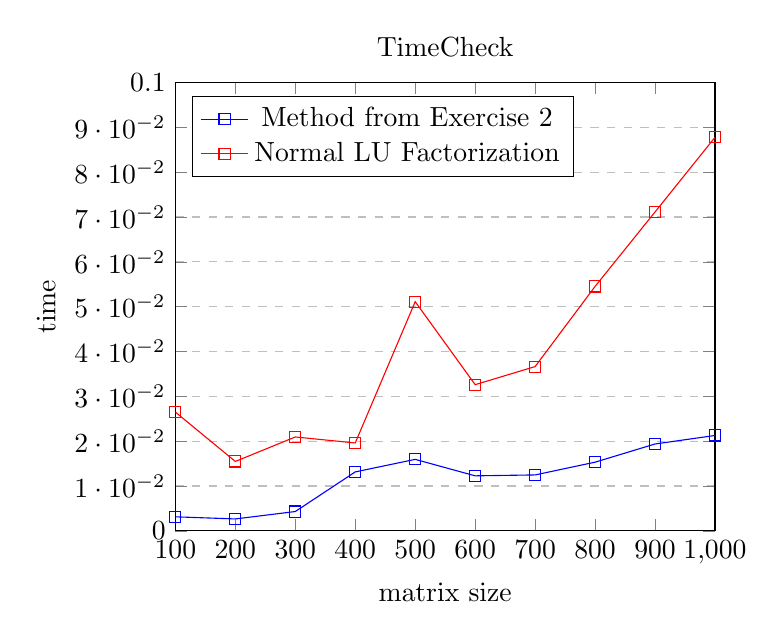
\begin{tikzpicture}
\begin{axis}[
    title={TimeCheck},
    xlabel={matrix size},
    ylabel={time},
    xmin=100, xmax=1000,
    ymin=0, ymax=0.1,
    xtick={100,200,300,400,500,600,700,800,900,1000},
    ytick={0,0.01,0.02,0.03,0.04,0.05,0.06,0.07,0.08,0.09,0.1},
    legend pos=north west,
    ymajorgrids=true,
    grid style=dashed,
]
 
\addplot[
    color=blue,
    mark=square,
    ]
    coordinates {
    (100, 0.003122)(200, 0.002649)(300, 0.004302)(400,0.013137)(500,0.015937)(600,0.012264)(700, 0.012467)(800, 0.015310)(900, 0.019368)(1000, 0.021267)
    };
\addplot[
    color=red,
    mark=square,
    ]
    coordinates {
    (100, 0.026487)(200, 0.015470)(300, 0.020934)(400,0.019596)(500,0.051112)(600,0.032600)(700, 0.036631)(800, 0.054510)(900, 0.071119)(1000, 0.087773)
    };    
\legend{Method from Exercise 2,Normal LU Factorization}


\end{axis}
\end{tikzpicture}
\end{document}
